% Copyright 2022 Pierre S. Caboche. All rights reserved.

\renewcommand{\currentPart}{ElasticSearch}
\part{\currentPart} \label{part - ElasticSearch}


In the previous parts, we saw the general concepts behind full-text search, lemmatisation, faceting, etc. We saw how to use Solr to generate some statistics about word usage in Japanese songs, and then we ran this tool on a few thousand songs from a variety of artists (part \ref{analysing-lyrics}). \\

Now we are going to do the same with ElasticSearch, currently the most popular enterprise search engine. \\

Many of the concepts we have seen so far also apply to ElasticSearch. The are, of course, a number of differences in terms of setup, configuration, syntax, etc. However, the general steps are the same (running the server, create the collection, input some documents, query the collection\dots) \\

Also, at every step of the way, we know what kind of result to expect since we have already done the same in Solr. \\





\section{Starting ElasticSearch} \label{starting-elasticsearch}

Like with Solr, we are going to run ElasticSearch (and other related tools) using Docker. \\



I tried to run the latest version of ElasticSearch (currently: 8.3.3) and followed the official documentation: \\
\url{https://www.elastic.co/guide/en/elasticsearch/reference/current/docker.html} \\

However, I (and other people on the internet) invariably ended up with the same error:
\begin{lstlisting}[language=sh]
ERROR: for kibana  Container "............" is unhealthy.
ERROR: Encountered errors while bringing up the project.
\end{lstlisting}

\bigskip
This is the reference guide for the latest version. Hopefully these issues would be resolved in the future (for version 8 or later). \\

So for this article, we will stick with ElasticSearch version 7.17.5. \\


\bigskip
\bigskip

Unlike Solr, the Kuromoji plugin is not installed by default in ElasticSearch. This means we needs to build a custom Docker image for ElasticSearch with Kuromoji installed. For this, we need a Dockerfile: \\

\texttt{es\_kuro/Dockerfile}
\lstinputlisting[language=sh]{files/bsd-licensed/es7/es_kuro/Dockerfile}


\bigskip

For better ease of use and access to other features, we will interact with ElasticSearch by using Kibana. This means we need to configure them to run together. \\

An easy way to do this is by using \texttt{docker-compose}: \\

\texttt{docker-compose.yml}
\lstinputlisting[language=sh]{files/bsd-licensed/es7/docker-compose.yml}

\bigskip

The docker \texttt{docker-compose.yml} file defines how the services will run together (in an isolated environment). \\

It also indicates that we need to build a custom Docker image for our ElasticSearch service (so that it comes with the kuromoji plugin installed, as seen in the previous step). \\

All this (and more) is described in the \texttt{docker-compose.yml} file. \\

\bigskip

Now all we need to do is run the following command:

\begin{lstlisting}[language=sh]
docker-compose up
\end{lstlisting}

\bigskip

From there, docker and docker-compose will take care of:
\begin{itemize}
	\item downloading the Docker images that we will need (ElasticSearch and Kibana, both at version 7.15.5)
	
	\item building our custom ElasticSearch
	
	\item running our services with the configuration specified in the file
\end{itemize}

\bigskip

If the previous command ran without issue, you should be able to connect to Kibana at the following URL:
\begin{center}
\url{http://localhost:5601}
\end{center}

\bigskip

To stop ElasticSearch and Kibana, just press \texttt{Ctrl + C} in the terminal where \texttt{docker-compose} is running. The servers will stop graciously. \\

Pressing \texttt{Ctrl + C} a second time will force ElasticSearch and Kibana to stop. \\



\bigskip


\section{Using Kibana}

If you followed the instructions from section \ref{starting-elasticsearch}, then Kibana should be running, and accessible at:
\begin{center}
	\url{http://localhost:5601}
\end{center}

\bigskip

Following this URL should lead you to Kibana's start page:

\begin{figure}[h]
	\centering
	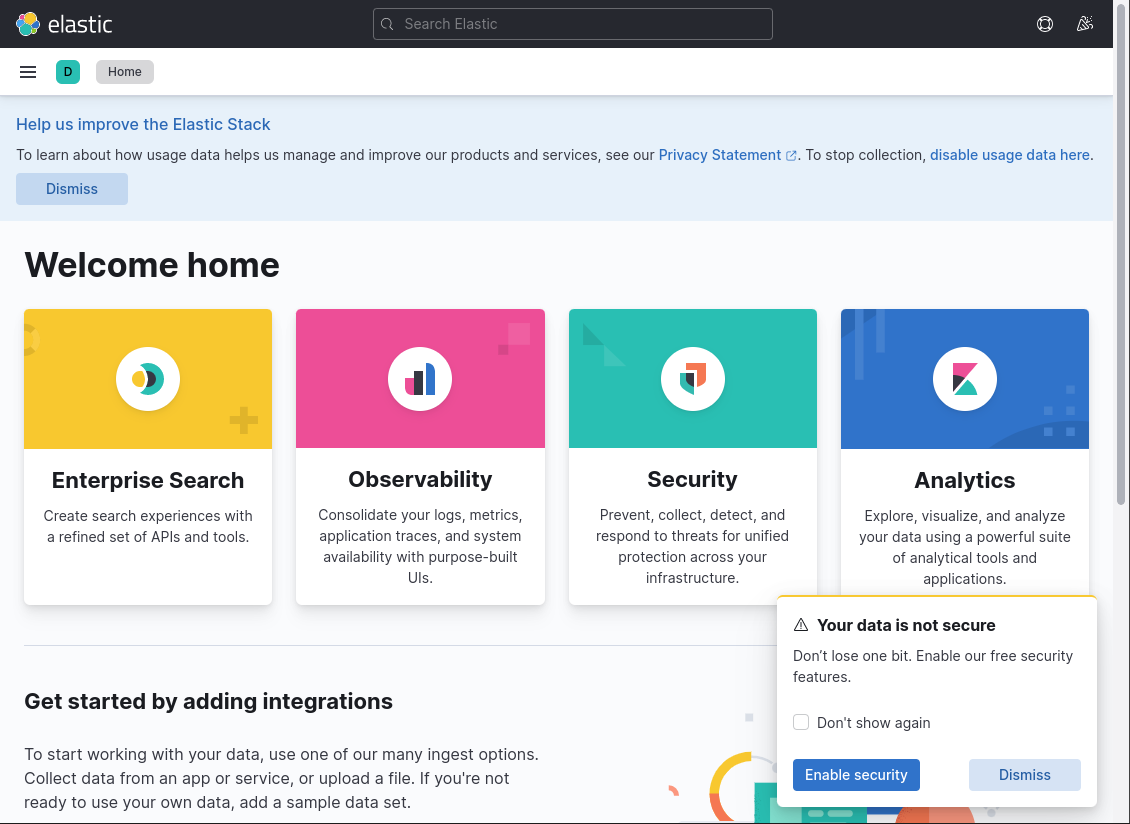
\includegraphics[width=0.8\linewidth]{files/images/kibana-start-page.png}
	\caption{Kibana's start page}
	\label{fig:kibana-start-page}
\end{figure}


\bigskip

From there, it is possible to explore the different Kibana components, import some sample datasets, create Dashboards\dots\ and learn more about Kibana and ElasticSearch in general. \\

\bigskip

For this article, we will only need to use the development tools from Kibana\dots \\

Note: we could use any tool that allows to perform HTTP requests to the ElasticSearch server, but Kibana comes with some extra features as well as auto-completion. \\


\newpage

To access Kibana's Dev Tools, click on the \emph{``hamburger"} menu (top left) >> then scroll down to ``Management" and select ``Dev Tools":


\begin{figure}[h]
	\centering
	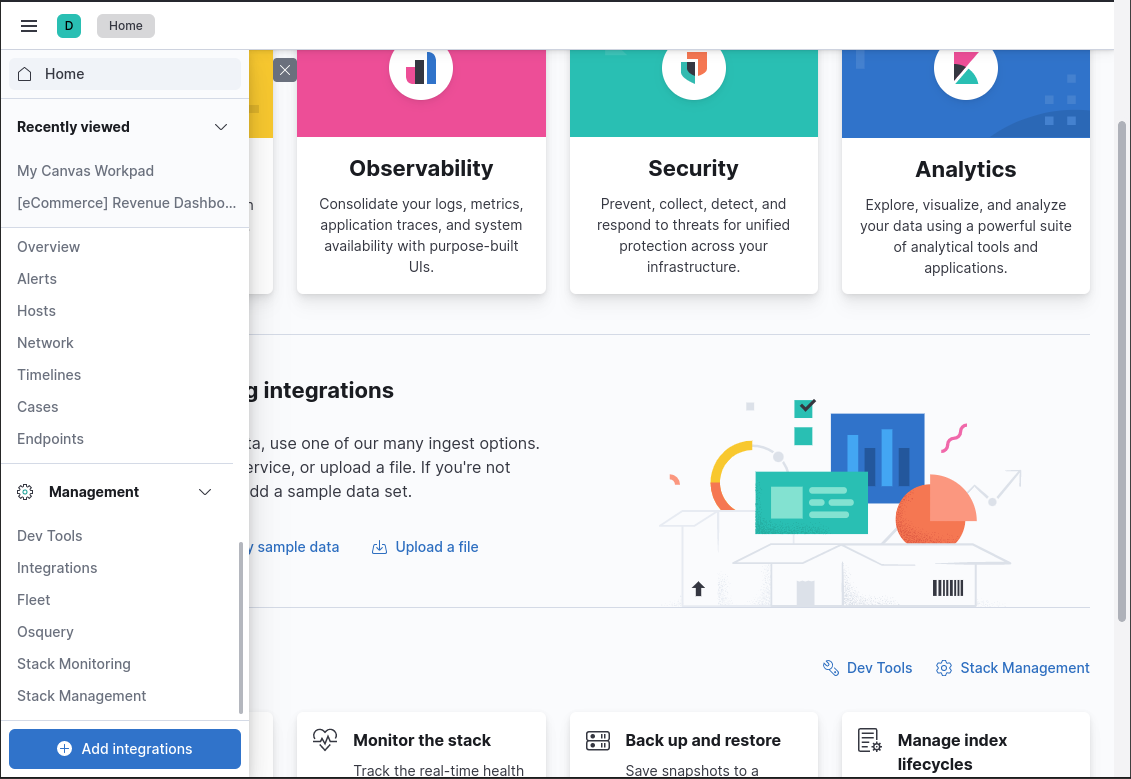
\includegraphics[width=0.8\linewidth]{files/images/kibana-menu}
	\caption{Menu to access Kibana's Dev Tools}
	\label{fig:access-kibana-dev-tools}
\end{figure}

\bigskip

This will lead you to the following screen:

\begin{figure}[h]
	\centering
	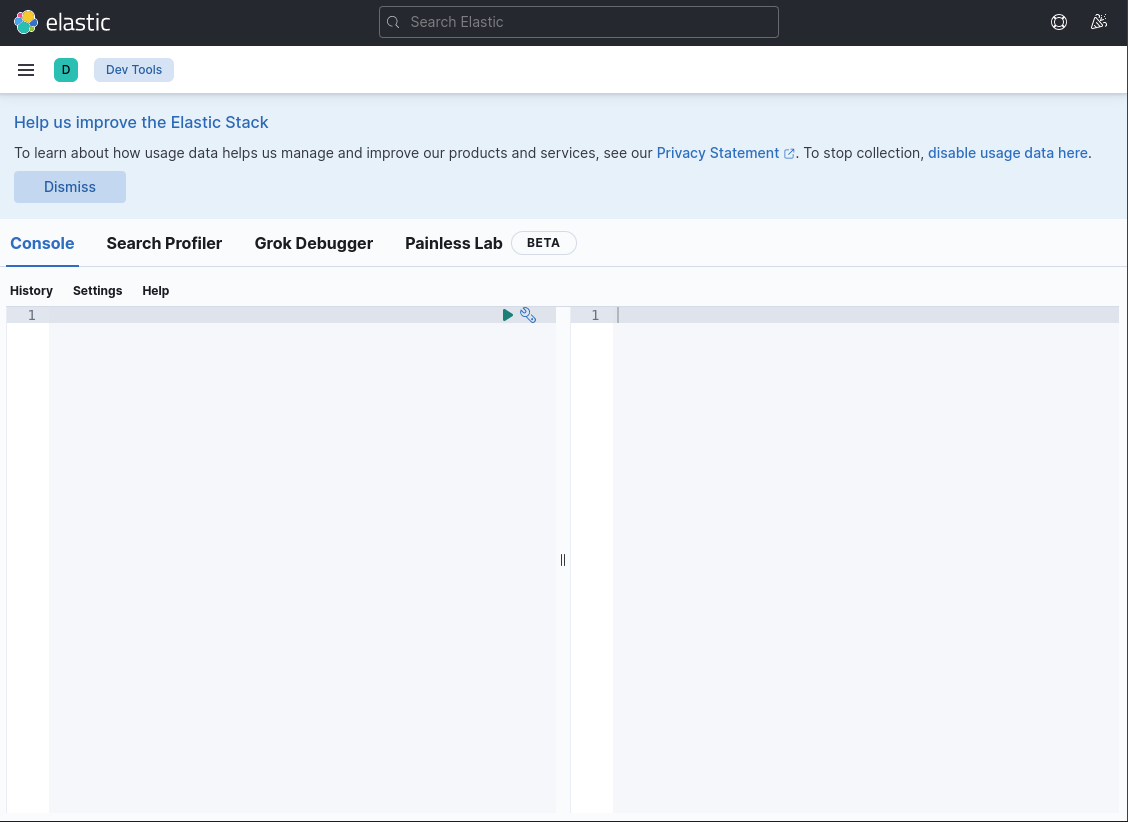
\includegraphics[width=0.8\linewidth]{files/images/kibana-dev-tools}
	\caption{Kibana's Dev Tools}
	\label{fig:kibana-dev-tools}
\end{figure}

\bigskip

On the left side, you can type the HTTP requests to send to ElasticSearch (we will see some examples in section \ref{using-elasticsearch}). The server's responses will be displayed on the right.

\newpage



\section{Using ElasticSearch} \label{using-elasticsearch}

\subsection{Testing that Kuromoji works} \label{es-testing-kuromoji}

The first thing we will do is see if the \kuromoji\ plugin works, by trying to process some text: \\

\begin{lstlisting}[language=sh]
POST _analyze
{
	"tokenizer": "kuromoji_tokenizer",
	"text": """普通の星の下に生まれ 普通の星の下を歩き
	普通の町で 君と出会って 特別な恋をする"""
	,
	"filter": 
	[
 "kuromoji_baseform"
	, "kuromoji_part_of_speech"
	, "cjk_width"
	, "ja_stop"
	, "kuromoji_stemmer"
	, "lowercase"
	]
}
\end{lstlisting}


\bigskip

The result is as follows (edited for brevity):

\begin{lstlisting}[language=sh]
{
	"tokens" : [
	{
		"token" : "普通",
		"start_offset" : 0,
		"end_offset" : 2,
		"type" : "word",
		"position" : 0
	},
	{
		"token" : "星",
		"start_offset" : 3,
		"end_offset" : 4,
		"type" : "word",
		"position" : 2
	},
	{
		"token" : "下",
		"start_offset" : 5,
		"end_offset" : 6,
		"type" : "word",
		"position" : 4
	},
	{
		"token" : "生まれる",
		"start_offset" : 7,
		"end_offset" : 10,
		"type" : "word",
		"position" : 6
	},
	{
		"token" : "普通",
		"start_offset" : 11,
		"end_offset" : 13,
		"type" : "word",
		"position" : 7
	},
	(...)
	]
}
\end{lstlisting}

\bigskip

So as you can see, the \kuromoji\ plugin works. We can also see the result of tokenisation (lexeme, offsets, type, position). \\





\subsection{Creating a core (collection)} \label{create-es-core}

Next, we create a core called \texttt{/song\_jp} : \\

\begin{lstlisting}[language=sh]
PUT /song_jp
{
	"settings": {
		"index": {
			"analysis": {
				"analyzer": {
					"jp_analyser": {
						"tokenizer": "kuromoji_tokenizer",
						"filter": 
						[
						"kuromoji_baseform"
						, "kuromoji_part_of_speech"
						, "cjk_width"
						, "ja_stop"
						, "kuromoji_stemmer"
						, "lowercase"
						]
					}
				}
			}
		}
	}
	,
	"mappings": {
		"dynamic_templates": [
		{
			"txt_japanese": {
				"match_mapping_type": "string",
				"match": "*_txt_ja",
				"mapping": {
					"type": "text",
					"analyzer": "jp_analyser",
					"term_vector": "with_positions_offsets",
					"store" : true,
					"fielddata":true
				}
			}
		}
		,
		{
			"str": {
				"match_mapping_type": "string",
				"match": "*_str",
				"mapping": {
					"type": "keyword"
				}
			}
		}
		]
	}
}
\end{lstlisting}




\bigskip

First we need to configure an analyser for text in Japanese. We need to give it a name: \texttt{jp\_analyser}. 

This analyser will use the \kuromoji\ tokeniser (\texttt{kuromoji\_tokenizer}). \\


\bigskip

\newpage

In Solr, we decided to use dynamic fields (section \ref{dynamic-fields}): 

\begin{itemize}
	\item \texttt{*\_txt\_jp} : fields of Solr type \texttt{text\_ja} (text which is tokenised by \kuromoji, and then indexed and stored)
	
	\item \texttt{*\_str} : fields of Solr type \texttt{strings} (string values that are compared ``as is"; ideal for: tags, categories, etc.)
\end{itemize}

\bigskip

We want to do the same with ElasticSearch:
\begin{itemize}
	\item \texttt{*\_txt\_jp} : fields of ElasticSearch type \texttt{text}, tokenised by \kuromoji, with positions and offsets, stored
	
	\item \texttt{*\_str} : fields of Solr type \texttt{keyword}
\end{itemize}


\bigskip
\bigskip

Finally, the {*\_txt\_jp} fields are declared with \texttt{"fielddata":true}. 

This is necessary to do some \aggregations\ on a field type \texttt{text} (as we will see in section \ref{aggregation-termsVectors}), but it uses more memory. \\

All these fields are defined in \texttt{"dynamic\_templates"}.


\bigskip
\bigskip



\subsection{Deleting a core (collection)}

If at any point you need to delete a core (e.g. to recreated it), perform the following action: \\

\begin{lstlisting}[language=sh]
DELETE /song_jp
\end{lstlisting}

\bigskip



\subsection{Adding a document}

Adding a document is done with the following HTTP request:

\begin{lstlisting}[language=sh]
POST /song_jp/_doc/1
{
	"band_str": "Band name",
	
	"lyrics_txt_ja": 
"""
The song lyrics go there...

(but because of copyright law, 
I cannot give you an actual example)

"""		
}
\end{lstlisting}

\bigskip

The document id is part of the URL (which means it must bne URL-encoded). \\


\bigskip
\bigskip
\bigskip

\subsection{Viewing the \texttt{termsVector}s of a document} \label{es-viewing-termsVector}

\bigskip
To view the \termsVector\ used in every field in the document, you can use the following HTTP request:

\begin{lstlisting}[language=sh]
GET /song_jp/_termvectors/1	
\end{lstlisting}

\bigskip
\dots or if you want the \termsVector\ of one field in particular:

\begin{lstlisting}[language=sh]
GET /song_jp/_termvectors/1?fields=lyrics_txt_ja	
\end{lstlisting}

\bigskip
\dots and you can be precise in your request:

\begin{lstlisting}[language=sh]
GET /song_jp/_termvectors/1?fields=lyrics_txt_ja
{
	"term_statistics": true,
	"field_statistics": true,
	"positions": false,
	"offsets": false,
	"filter": {
		"max_num_terms": 10,
		"min_term_freq": 1,
		"min_doc_freq": 1
	}
}
\end{lstlisting}


\bigskip
\bigskip

These queries allow to inspect the \termsVector s, and the type of information they contain. \\

Result example (edited for brevity):

\begin{lstlisting}[language=sh]
{
	"_index" : "song_jp",
	"_type" : "_doc",
	"_id" : "1",
	"_version" : 1,
	"found" : true,
	"took" : 0,
	"term_vectors" : {
		"lyrics_txt_ja" : {
			"field_statistics" : {
				"sum_doc_freq" : 130,
				"doc_count" : 3,
				"sum_ttf" : 276
			},
			"terms" : {
				"いける" : {
					"term_freq" : 1,
					"tokens" : [
					{
						"position" : 6,
						"start_offset" : 12,
						"end_offset" : 14
					}
					]
				},
				(...)
			
			        "愛する" : {
				"term_freq" : 4,
				"tokens" : [
				{
					"position" : 108,
					"start_offset" : 208,
					"end_offset" : 211
				},
				{
					"position" : 193,
					"start_offset" : 353,
					"end_offset" : 356
				},
				{
					"position" : 199,
					"start_offset" : 363,
					"end_offset" : 366
				},
				{
					"position" : 205,
					"start_offset" : 373,
					"end_offset" : 376
				}
				]
			},
			(...)
		}
	}
}
\end{lstlisting}



\bigskip
\bigskip
\bigskip



\subsection{Aggregation on \texttt{termsVectors}} \label{aggregation-termsVectors}

Now we reach the part where we want to answer questions of the type: \emph{``Which words are the most used in (a certain result-set) ?"} \\

As we have seen many times in section \emph{\longref{exploring-dataset}}, this is done with an aggregation on a text field containing \termsVector s (and \texttt{fielddata}). \\

\begin{lstlisting}[language=sh]
GET /song_jp/_search
{
	"size": 0,
	"aggs": {
		"test": {
			"terms": {
				"field": "lyrics_txt_ja",
				"size": 100
			}
		}
	}
}
\end{lstlisting}

This query is only possible if the field used in the \faceting\ has been declared with \texttt{"fielddata": true} . \\

If the \texttt{"fielddata"} was not set, then we would be met with the following error:

\begin{lstlisting}[language=sh]
“Fielddata is disabled on text fields by default. Set `fielddata=true` on [`your_field_name`] in order to load field data in memory by uninverting the inverted index. Note that this can however, use “significant memory.” – if this happens you can either enable the field-data on that text field, or choose another way to query the data (again, because field-data consumes a lot of memory and is not recommended).
\end{lstlisting}

\bigskip
\bigskip

We are more interested in the result of the aggregation (list of terms) than the list of documents. So we set the \texttt{size} of the result-set (list of documents) to 0. \\

Then we specify the \texttt{size} of the aggregation to the number of terms we want to display (default value: 10). \\


\bigskip
\bigskip
\bigskip

The result looks something like this:

\begin{lstlisting}[language=sh]
{
	"took" : 24,
	"timed_out" : false,
	"_shards" : {
		"total" : 1,
		"successful" : 1,
		"skipped" : 0,
		"failed" : 0
	},
	"hits" : {
		"total" : {
			"value" : 3,
			"relation" : "eq"
		},
		"max_score" : null,
		"hits" : [ ]
	},
	"aggregations" : {
		"test" : {
			"doc_count_error_upper_bound" : 0,
			"sum_other_doc_count" : 109,
			"buckets" : [
			{
				"key" : "時",
				"doc_count" : 3
			},
			{
				"key" : "何",
				"doc_count" : 2
			},
			{
				"key" : "僕",
				"doc_count" : 2
			},
			{
				"key" : "君",
				"doc_count" : 2
			},
			(...)
			
			]
		}
	}
}
\end{lstlisting}


\bigskip
\bigskip


%\newpage

\subsection{ElasticSearch's ``More Like This"}

We have talked about the \MLT\ queries, and show how to run them in Solr in section \emph{\longref{mlt}}. \\


Performing a \MLT\ query in ElasticSearch is easy. Here is an example with one document:

\newpage

\begin{lstlisting}[language=sh]
GET /_search
{
	"query": {
		"more_like_this": {
			"fields": [ "lyrics_txt_ja" ],
			"like": [
			{
				"_index": "song_jp",
				"_id": "1"
			}        
			],
			"min_term_freq": 1,
			"max_query_terms": 12
		}
	}
}
\end{lstlisting}

\bigskip


It is also possible to perform a \MLT\ query on more than one document, and also one custom text:

\begin{lstlisting}[language=sh]
GET /_search
{
	"query": {
		"more_like_this": {
			"fields": [ "lyrics_txt_ja" ],
			"like": [
			{
				"_index": "song_jp",
				"_id": "1"
			}        
			],
			{
				"_index": "song_jp",
				"_id": "2"
			},
			"You can also perform a 'More Like This' query on custom text, not just on documents."
			],
			"min_term_freq": 1,
			"max_query_terms": 12
		}
	}
}
\end{lstlisting}

\bigskip

A notable difference with Solr: in ElasticSearch, you can pass a list of documents or custom strings on which to run the \MLT\ query, whereas in Solr you pass a query (which may return one or more documents) and the \MLT\ feature is run on the result of this query (as shown in section \ref{mlt-solr-example}). \\

On one hand, Solr allows you to run \MLT\ on the result of a query. On the other hand,  ElasticSearch allows you to run \MLT\ on a custom query. \\

In practice though, you would rarely want to run a \MLT\ query on more than one document (because the results become less relevant). Being able to run \MLT\ on a custom string can be convenient. \\



\url{https://www.elastic.co/guide/en/elasticsearch/reference/current/query-dsl-mlt-query.html}




